%% source: 2023-sp-redemption_midterm_02
\begin{prob}
    Suppose a DFS is run on the graph shown below using node 11 as the source.

    \begin{center} 
        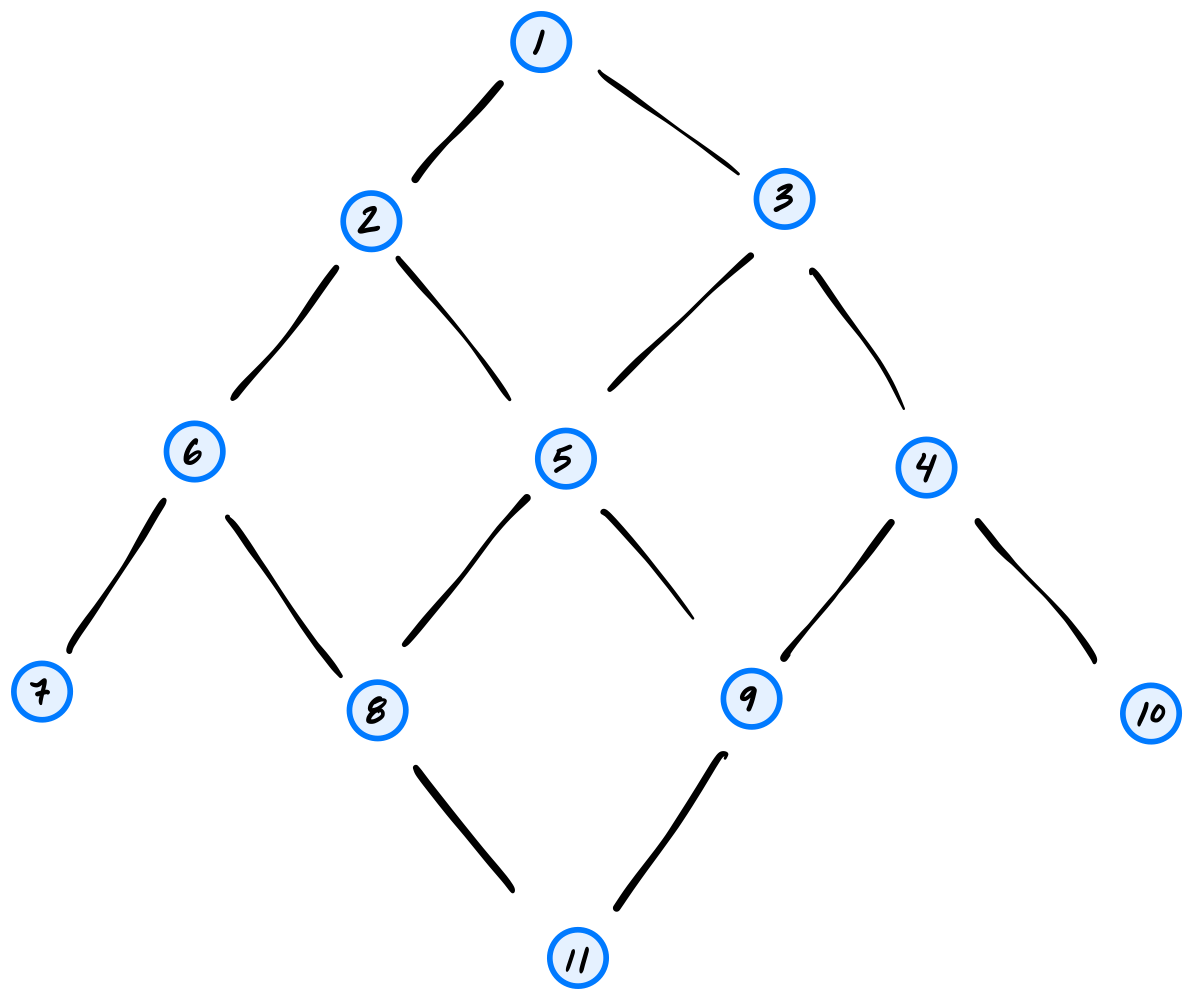
\includegraphics[width=.6\textwidth]{./fig/g2.png}
    \end{center}

    What will be the DFS predecessor of node 3 in the search? Use the convention that a node's
    neighbors are produced in ascending order by label.

    \inlineresponsebox[.75in]{1}

\end{prob}
